\section*{Ejercicio \#3}
En esta sección se presenta gráficas comparativas, evaluando el tiempo (en segundos) vs la cantidad de elementos a ordenar (la cantidad máxima de datos a ordenar es de 200 000). Para obtener un resultado con menor cantidad de fallas, cada algoritmo fue probado con datos aleatorios 3 veces y promediando los resultados de estos.
\subsection*{Por algoritmo de ordenamiento}
Para esta parte se probaron cada uno de los algoritmos de ordenamiento de acuerdo al lenguaje de programación (C++, Java y Python), permitiendo obtener que lenguaje es más eficiente frente a los otros de acuerdo al algoritmo.

\subsubsection*{BubbleSort}
\begin{figure}[H]
	   \centering
	   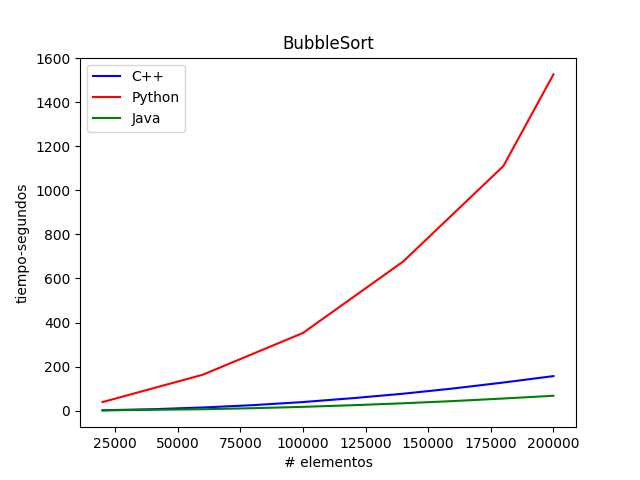
\includegraphics[scale=0.5]{Practica01/images/plots/BubbleSort.png}
	   \label{imgBubble}
	   \caption{Gráfica del algoritmo Bubble Sort implementado en C++,Python y Java evaluando de 20000 hasta 200000 datos}
\end{figure}
%En la gráfica \ref{imgBubble} se aprecia que?? Python es mas lento??Estoy buscando una explicación

\subsubsection*{CountingSort}
\begin{figure}[H]
	   \centering
	   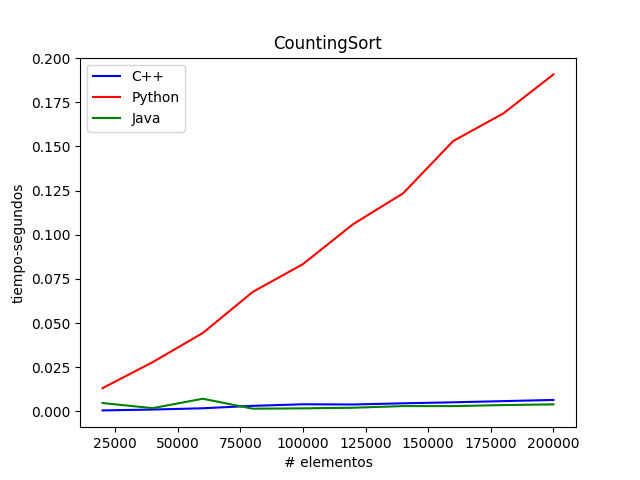
\includegraphics[scale=0.5]{Practica01/images/plots/CountingSort.png}
	   \caption{Gráfica del algoritmo Counting Sort implementado en C++,Python y Java evaluando de 20000 hasta 200000 datos}
\end{figure}
\subsubsection*{HeapSort}
\begin{figure}[H]
	   \centering
	   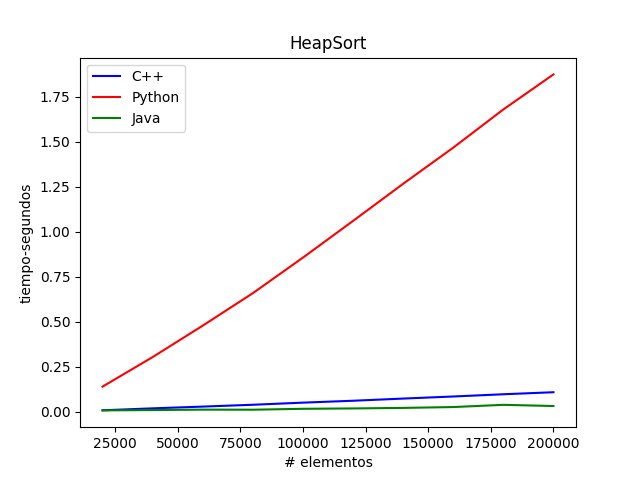
\includegraphics[scale=0.5]{Practica01/images/plots/HeapSort.png}
	   \caption{Gráfica del algoritmo Heap Sort implementado en C++,Python y Java evaluando de 20000 hasta 200000 datos}
\end{figure}
\subsubsection*{InsertionSort}
\begin{figure}[H]
	   \centering
	   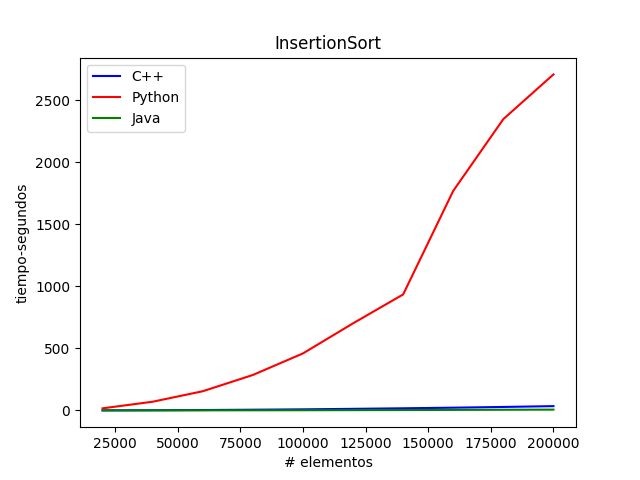
\includegraphics[scale=0.5]{Practica01/images/plots/InsertionSort.png}
	   \caption{Gráfica del algoritmo Insertion Sort implementado en C++,Python y Java evaluando de 20000 hasta 200000 datos}
\end{figure}
\subsubsection*{MergeSort}
\begin{figure}[H]
	   \centering
	   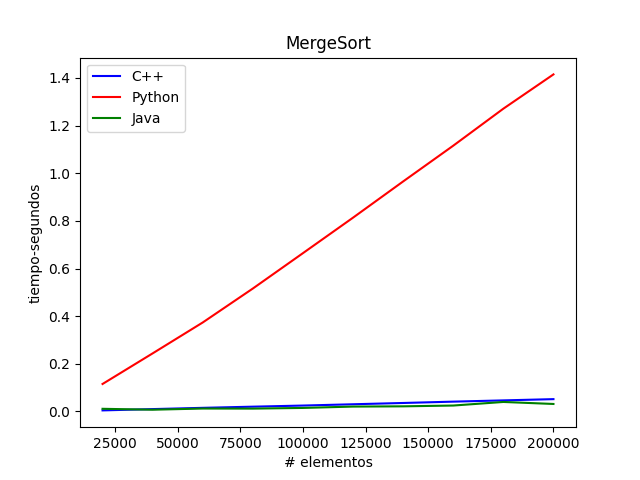
\includegraphics[scale=0.5]{Practica01/images/plots/MergeSort.png}
	   \caption{Gráfica del algoritmo Merge Sort implementado en C++,Python y Java evaluando de 20000 hasta 200000 datos}
\end{figure}
\subsubsection*{QuickSort}
\begin{figure}[H]
	   \centering
	   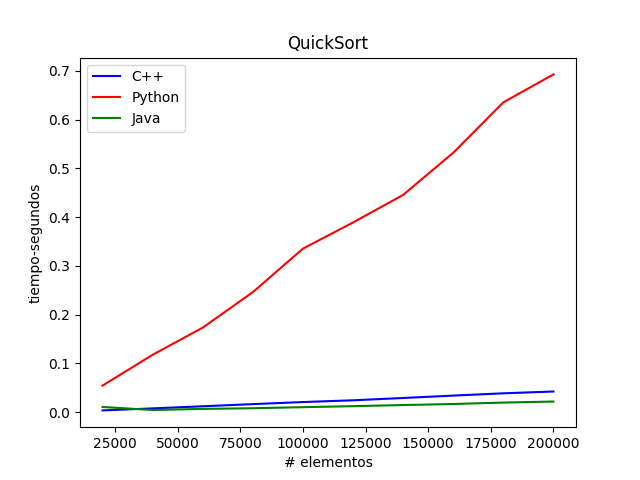
\includegraphics[scale=0.5]{Practica01/images/plots/QuickSort.png}
	   \caption{Gráfica del algoritmo Quick Sort implementado en C++,Python y Java evaluando de 20000 hasta 200000 datos}
\end{figure}
\subsubsection*{SelectionSort}
\begin{figure}[H]
	   \centering
	   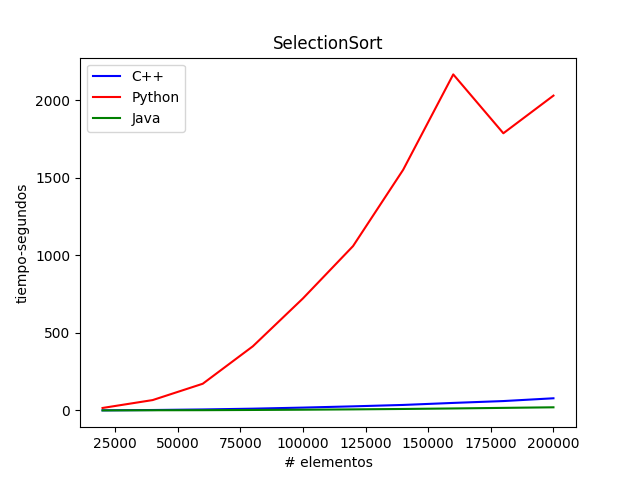
\includegraphics[scale=0.5]{Practica01/images/plots/SelectionSort.png}
	   \caption{Gráfica del algoritmo Selection Sort implementado en C++,Python y Java evaluando de 20000 hasta 200000 datos}
\end{figure}

\subsubsection*{Conclusión}
Hemos podido observar que el lenguaje de programación menos eficiente en procesar los doscientos mil datos es \verb!Python!. Ya que a la hora de correr un programa, se realiza la ejecución línea por línea envés de ser compilada a código máquina como \verb!C++!; otros lenguajes como \verb!Java! corren también más rápido a comparación de \verb!Python!, ya que incluyen un compilador JIT, el cuál sólo necesita traducir de bytecode a código máquina.

De acuerdo a Guido Van-Rossum, creador del lenguaje \verb!Python!, para evaluar una expresión como $a+b$, primero debe inspeccionar los objetos para saber de que tipo son. Luego se invoca la operación sobrecargada de adición (que puede ser para cadenas o números). En cambio \verb!Java! puede realizar una adición eficiente en enteros o números de punto flotante restando así tiempo en su ejecución.\cite{guido}

\subsection*{Por lenguaje de programación}
Para esta parte se probaron todos los algoritmos de ordenamiento obteniendo una gráfica por lenguaje de programación, permitiendo verificar que algoritmo es más eficiente.
\begin{itemize}
    \item \textbf{C++}
        \begin{figure}[H]
	        \centering
	        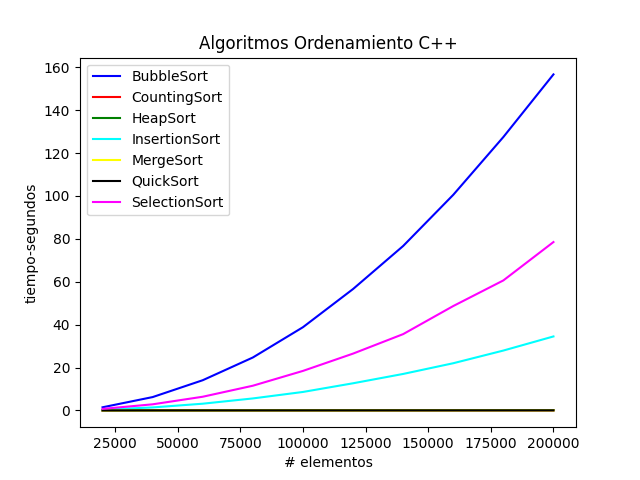
\includegraphics[scale=0.5]{Practica01/images/plots/Sorts_C++.png}
	        \caption{Gráfica de los algoritmos de ordenamiento implementados en C++, evaluando de 20000 hasta 200000 datos}
		\end{figure}
En la gráfica se aprecia que el algoritmo más lento para ordenar un array es el Bubble Sort, seguido del Selection Sort y el Insertion Sort.
        \begin{figure}[H]
	        \centering
	        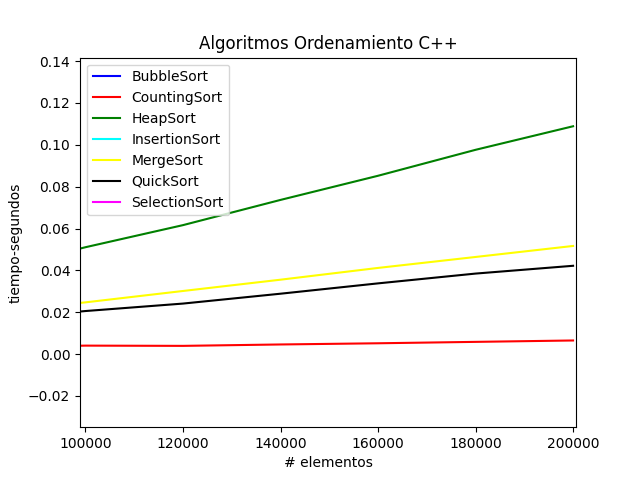
\includegraphics[scale=0.5]{Practica01/images/plots/Sorts2_C++.png}
	        \caption{Gráfica con acercamiento de los algoritmos de ordenamiento implementados en C++, evaluando de 100000 hasta 200000 datos}
		\end{figure}
En la gráfica con acercamiento se aprecia que el algoritmo más eficiente para ordenar un array es el Counting Sort, seguido del Quick Sort, el Merge Sort y el Heap Sort.
    \item \textbf{Python}
        \begin{figure}[H]
	        \centering
	        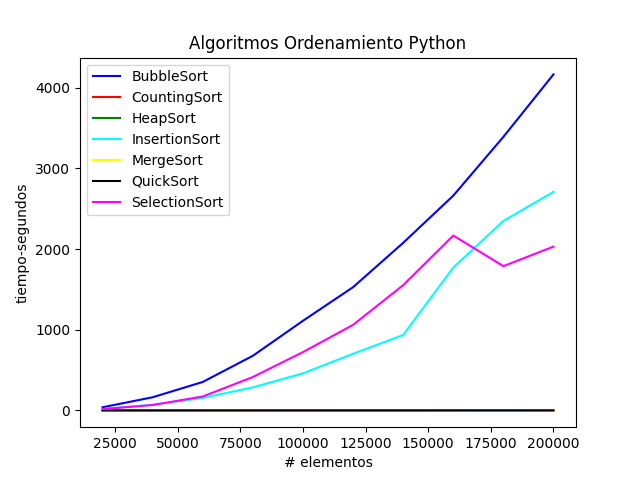
\includegraphics[scale=0.5]{Practica01/images/plots/Sorts_Python.png}
	        \caption{Gráfica de los algoritmos de ordenamiento implementados en Python, evaluando de 20000 hasta 200000 datos}
		\end{figure}
En la gráfica se aprecia que el algoritmo más lento para ordenar un array es el Bubble Sort, seguido del Selection Sort y el Insertion Sort.
        \begin{figure}[H]
	        \centering
	        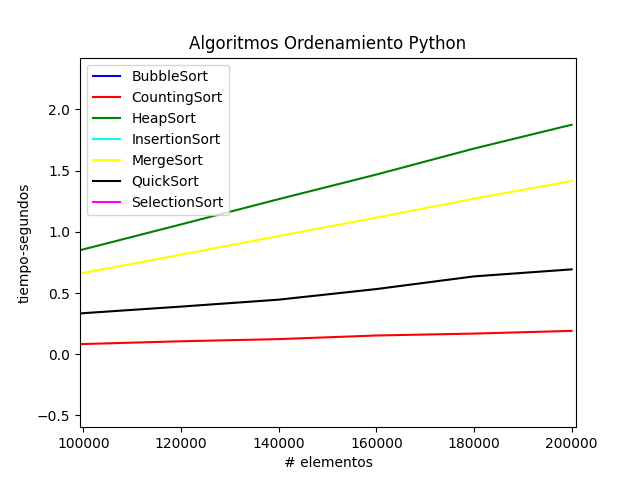
\includegraphics[scale=0.5]{Practica01/images/plots/Sorts2_Python.png}
	        \caption{Gráfica con acercamiento de los algoritmos de ordenamiento implementados en Python, evaluando de 100000 hasta 200000 datos}
		\end{figure}
En la gráfica con acercamiento se aprecia que el algoritmo más eficiente para ordenar un array es el Counting Sort, seguido del Quick Sort, el Merge Sort y el Heap Sort.
    \item \textbf{Java}
        \begin{figure}[H]
	        \centering
	        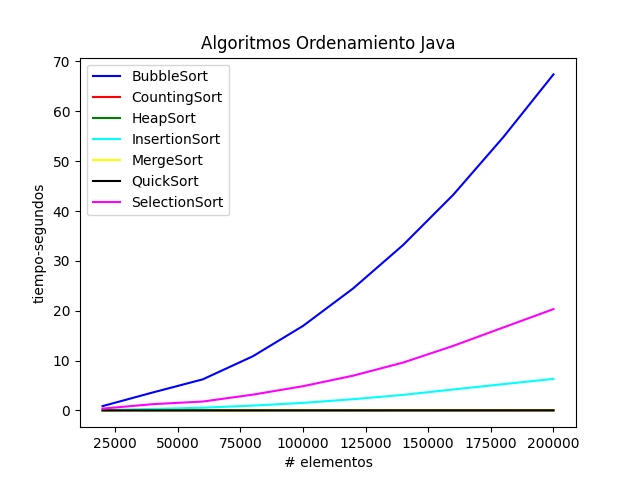
\includegraphics[scale=0.5]{Practica01/images/plots/Sorts_Java.png}
	        \caption{Gráfica de los algoritmos de ordenamiento implementados en Java, evaluando de 20000 hasta 200000 datos}
		\end{figure}
En la gráfica se aprecia que el algoritmo más lento para ordenar un array es el Bubble Sort, seguido del Selection Sort y el Insertion Sort.
        \begin{figure}[H]
	        \centering
	        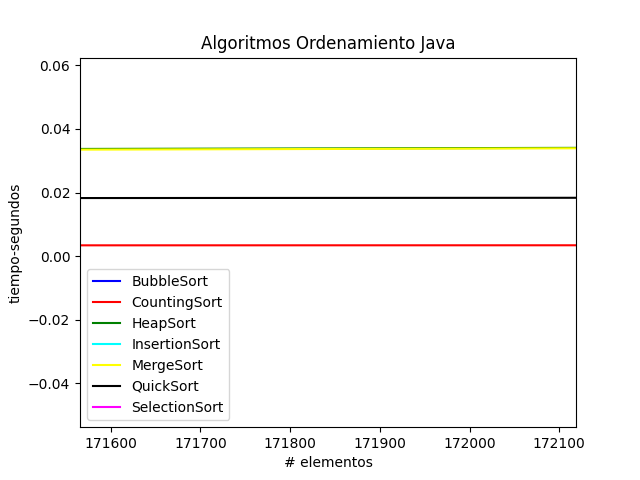
\includegraphics[scale=0.5]{Practica01/images/plots/Sorts2_Java.png}
	        \caption{Gráfica con acercamiento de los algoritmos de ordenamiento implementados en Java, evaluando de 100000 hasta 200000 datos}
		\end{figure}
En la gráfica con acercamiento se aprecia que el algoritmo más eficiente para ordenar un array es el Counting Sort, seguido del Quick Sort, el Merge Sort y el Heap Sort.
\end{itemize}

\subsubsection*{Conclusión}
Como hemos visto en todos los lenguajes, el algoritmo de ordenamiento ganador es el Counting Sort con una complejidad algorítmica de $O(n+k)$, siendo $n$ la cantidad de datos a ordenar y $k$ el tamaño del vector auxiliar (máximo - mínimo), a la vez tiene como limitación que solo ordena números enteros, no vale para ordenar cadenas y no se aconseja para ordenar números decimales; QuickSort obtuvo el segundo lugar en este experimento, cuya complejidad es $O(nlogn)$, siendo uno de los más usados, la parte negativa va a depender de la distribución de los datos y la elección de pivote.
% ajá
% ok, creo que ya está
% Y la parte negativa del counting sort .Cual seria?
% no lo sé
% like
% confirmo
% ya lo subimos tons?
%Pregunta en el grupo , que todos revisen 
% dime 
% oka 
% chau
% chau :)
Para escoger un algoritmo de ordenamiento, podemos considerar el tiempo de ejecución, la complejidad en espacio y el formato esperado de la entrada (ya sea si está parcialmente ordenado).

El repositorio del trabajo se encuentra en \href{https://github.com/syordya/CSUNSA-EDA}{GitHub}\cite{repo}.

\iffalse
% ---- Para poner dos imágenes (una a lado de otra) ----
Como se muestra en la figuras \ref{fig:act-1_a} y \ref{fig:act-1_b}.
\begin{figure}[H]
\centering
\begin{minipage}{0.45\textwidth}
  \centering
  \includegraphics[width=0.9\textwidth]{act-1_a}
  \caption{Envío de \textit{ICMP ECHO REQUEST} de PC0 a PC1, PC2 y PC3.}
  \label{fig:act-1_a}
\end{minipage}\hfill
\begin{minipage}{0.45\textwidth}
  \centering
  \includegraphics[width=0.9\textwidth]{act-1_b}
  \caption{Respuesta de PC1, PC2 y PC3. Tabla ARP de PC0.}
  \label{fig:act-1_b}
\end{minipage}
\end{figure}
% ---- Para colocar una imagen ----
Como se muestra en la figura \ref{fig:act-3}
\begin{figure}[H]
  \centering
  \includegraphics[width=0.8\textwidth]{act-3}
  \caption{Tabla de subneteo para la red 192.168.100.0.}
  \label{fig:act-3}
\end{figure}
\fi